% В этом файле следует писать текст работы, разбивая его на
% разделы (section), подразделы (subsection) и, если нужно,
% главы (chapter).

% Предварительно следует указать необходимую информацию
% в файле SETUP.tex

%% В этот файл не предполагается вносить изменения

% В этом файле следует указать информацию о себе
% и выполняемой работе.

\documentclass [fontsize=14pt, paper=a4, pagesize, DIV=calc]%
{scrreprt}
% ВНИМАНИЕ! Для использования глав поменять
% scrartcl на scrreprt

% Здесь ничего не менять
\usepackage [T2A] {fontenc}   % Кириллица в PDF файле
\usepackage [utf8] {inputenc} % Кодировка текста: utf-8
\usepackage [russian] {babel} % Переносы, лигатуры

%%%%%%%%%%%%%%%%%%%%%%%%%%%%%%%%%%%%%%%%%%%%%%%%%%%%%%%%%%%%%%%%%%%%%%%%
% Создание макроса управления элементами, специфичными
% для вида работы (курс., бак., маг.)
% Здесь ничего не менять:
\usepackage{ifthen}
\newcounter{worktype}
\newcommand{\typeOfWork}[1]
{
	\setcounter{worktype}{#1}
}

% ВНИМАНИЕ!
% Укажите тип работы: 0 - курсовая, 1 - бак., 2 - маг.,
% 3 - бакалаврская с главами.
\typeOfWork{2}
% Считается, что курсовая и бак. бьются на разделы (section) и
% подразделы (subsection), а маг. — на главы (chapter), разделы и
%  подразделы. Если хочется,
% чтобы бак. была с главами (например, если она большая),
% надо выбрать опцию 3.

% Если при выборе 2 или 3 вы забудете поменять класс
% документа на scrreprt (см. выше, в самом начале),
% то получите ошибку:
% ./aux/appearance.tex:52: Package scrbase Error: unknown option ` chapterprefix=

%%%%%%%%%%%%%%%%%%%%%%%%%%%%%%%%%%%%%%%%%%%%%%%%%%%%%%%%%%%%%%%%%%%%%%%%
% Информация об авторе и работе для титульной страницы

\usepackage {titling}

% Имя автора в именительном падеже (для маг.)
\newcommand {\me}{%
А.\,С.~Коваленко%
}

% Имя автора в родительном падеже (для курсовой и бак.)
\newcommand {\byme}{%
А.\,С.~Коваленко%
}

% Любимый научный руководитель
\newcommand{\supervisor}%
{учёная степень, учёное звание /  должность И. О. Фамилия}

% идентифицируем пол (только для курсовой и бак.)
\newcommand{\bystudent}{
Студента %Студентки % Для курсовой: с большой буквы
}

% Год публикации
\date{2020}

% Название работы
\title{Обучение шумоподавляющей нейронной сети без использования чистых данных}

% Кафедра
%
\newboolean{needchair}
\setboolean{needchair}{false} % на ФИИТ не пишется (false), на ПМИ есть (true)

\newcommand {\thechair} {%
Кафедра компьютерного и аналогового моделирования светлого будущего%
}

\newcommand {\direction} {%
Направление подготовки\\
Фундаментальная информатика и информационные технологии%
}% Прикладная математика и информатика

%%%%%%%%%%%%%%%%%%%%%%%%%%%%%%%%%%%%%%%%%%%%%%%%%%%%%%%%%%%%%%%%%%%%%%%%
% Другие настраиваемые элементы текста

% Листинги с исходным кодом программ: укажите язык программирования
\usepackage{listings}
\lstset{
    language=[ISO]C++,%  Язык указать здесь
    basicstyle=\small\ttfamily,
    breaklines=true,%
    showstringspaces=false%
    inputencoding=utf8x%
}
% полный список языков, поддерживаемых данным пакетом, есть,
% например, здесь (стр. 13):
% ftp://ftp.tex.ac.uk/tex-archive/macros/latex/contrib/listings/listings.pdf

% Нумерация списков: можно при необходимести
% изменять вид нумерации (например, добавлять правую скобку).
% По умолчанию буду списки вида:
% 1.
% 2.
% Изменять вид нумерации можно в начале нумерации:
% \begin{enumerate}[1)] (В квадратных скобках указан желаемый вид)
\usepackage[shortlabels]{enumitem}
                    \setlist[enumerate, 1]{1.}

% Гиперссылки: настройте внешний вид ссылок
\usepackage%
[pdftex,unicode,pdfborder={0 0 0},draft=false,%backref=page,
    hidelinks, % убрать, если хочется видеть ссылки: это
               % удобно в PDF файле, но не должно появиться на печати
    bookmarks=true,bookmarksnumbered=false,bookmarksopen=false]%
{hyperref}


\usepackage {amsmath}      % Больше математики
\usepackage {amssymb}
\usepackage {textcase}     % Преобразование к верхнему регистру
\usepackage {indentfirst}  % Красная строка первого абзаца в разделе

\usepackage {fancyvrb}     % Листинги: определяем своё окружение Verb
\DefineVerbatimEnvironment% с уменьшенным шрифтом
	{Verb}{Verbatim}
	{fontsize=\small}

% Вставка рисунков
\usepackage {graphicx}

% Общее оформление
% ----------------------------------------------------------------
% Настройка внешнего вида

%%% Шрифты

% если закомментировать всё — консервативная гарнитура Computer Modern
\usepackage{paratype} % профессиональные свободные шрифты
%\usepackage {droid}  % неплохие свободные шрифты от Google
%\usepackage{mathptmx}
%\usepackage {mmasym}
%\usepackage {psfonts}
%\usepackage{lmodern}
%var1: lh additions for bold concrete fonts
%\usepackage{lh-t2axccr}
%var2: the package below could be covered with fd-files
%\usepackage{lh-t2accr}
%\usepackage {pscyr}

% Геометрия текста

\usepackage{setspace}       % Межстрочный интервал
\onehalfspacing

\newlength\MyIndent
\setlength\MyIndent{1.25cm}
\setlength{\parindent}{\MyIndent} % Абзацный отступ
\frenchspacing            % Отключение лишних отступов после точек
\KOMAoptions{%
    DIV=calc,         % Пересчёт геометрии
    numbers=endperiod % точки после номеров разделов
}

                            % Консервативный вариант:
%\usepackage                % ручное задание геометрии
%[%                         % (не рекомендуется в проф. типографии)
%  margin = 2.5cm,
  %includefoot,
  %footskip = 1cm
%] %
%  {geometry}

%%% Заголовки

\ifthenelse{\equal{\theworktype}{2}}{%
\KOMAoptions{%
    numbers=endperiod,% точки после номеров разделов
    headings=normal,   % размеры заголовков поменьше стандартных
    chapterprefix=true,% Печатать слово Глава в магистерской
    appendixprefix=true% Печатать слово Приложение
}
}

% шрифт для оформления глав и названия содержания
\newcommand{\SuperFont}{\Large\sffamily\bfseries}

% Заголовок главы
\ifthenelse{\value{worktype} > 1}{%
\renewcommand{\SuperFont}{\Large\normalfont\sffamily}
\newcommand{\CentSuperFont}{\centering\SuperFont}
\usepackage{fncychap}
\ChNameVar{\SuperFont}
\ChNumVar{\CentSuperFont}
\ChTitleVar{\CentSuperFont}
\ChNameUpperCase
\ChTitleUpperCase
}

% Заголовок (под)раздела с абзацного отступа
\addtokomafont{sectioning}{\hspace{\MyIndent}}

\renewcommand*{\captionformat}{~---~}
\renewcommand*{\figureformat}{Рисунок~\thefigure}

% Плавающие листинги
\usepackage{float}
\floatstyle{ruled}
\floatname{ListingEnv}{Листинг}
\newfloat{ListingEnv}{htbp}{lol}[section]

% точка после номера листинга
\makeatletter
\renewcommand\floatc@ruled[2]{{\@fs@cfont #1.} #2\par}
\makeatother


%%% Оглавление
\usepackage{tocloft}

% шрифт и положение заголовка
\ifthenelse{\value{worktype} > 1}{%
\renewcommand{\cfttoctitlefont}{\hfil\SuperFont\MakeUppercase}
}{
\renewcommand{\cfttoctitlefont}{\hfil\SuperFont}
}

% слово Глава
\usepackage{calc}
\ifthenelse{\value{worktype} > 1}{%
\renewcommand{\cftchappresnum}{Глава }
\addtolength{\cftchapnumwidth}{\widthof{Глава }}
}

% Очищаем оформление названий старших элементов в оглавлении
\ifthenelse{\value{worktype} > 1}{%
\renewcommand{\cftchapfont}{}
\renewcommand{\cftchappagefont}{}
}{
\renewcommand{\cftsecfont}{}
\renewcommand{\cftsecpagefont}{}
}

% Точки после верхних элементов оглавления
\renewcommand{\cftsecdotsep}{\cftdotsep}
%\newcommand{\cftchapdotsep}{\cftdotsep}

\ifthenelse{\value{worktype} > 1}{%
    \renewcommand{\cftchapaftersnum}{.}
}{}
\renewcommand{\cftsecaftersnum}{.}
\renewcommand{\cftsubsecaftersnum}{.}
\renewcommand{\cftsubsubsecaftersnum}{.}

%%% Списки (enumitem)

\usepackage {enumitem}      % Списки с настройкой отступов
\setlist %
{ %
  leftmargin = \parindent, itemsep=.5ex, topsep=.4ex
} %

% По ГОСТу нумерация должны быть буквами: а, б...
%\makeatletter
%    \AddEnumerateCounter{\asbuk}{\@asbuk}{м)}
%\makeatother
%\renewcommand{\labelenumi}{\asbuk{enumi})}
%\renewcommand{\labelenumii}{\arabic{enumii})}

%%% Таблицы: выбрать более подходящие

\usepackage{booktabs} % считаются наиболее профессионально выполненными
%\usepackage{ltablex}
%\newcolumntype {L} {>{---}l}

%%% Библиография

\usepackage{csquotes}        % Оформление списка литературы
\usepackage[
  backend=biber,
  hyperref=auto,
  sorting=none, % сортировка в порядке встречаемости ссылок
  language=auto,
  citestyle=gost-numeric,
  bibstyle=gost-numeric
]{biblatex}
\addbibresource{biblio.bib} % Файл с лит.источниками

% Настройка величины отступа в списке
\ifthenelse{\value{worktype} < 2}{%
\defbibenvironment{bibliography}
  {\list
     {\printtext[labelnumberwidth]{%
    \printfield{prefixnumber}%
    \printfield{labelnumber}}}
     {\setlength{\labelwidth}{\labelnumberwidth}%
      \setlength{\leftmargin}{\labelwidth}%
      \setlength{\labelsep}{\dimexpr\MyIndent-\labelwidth\relax}% <----- default is \biblabelsep
      \addtolength{\leftmargin}{\labelsep}%
      \setlength{\itemsep}{\bibitemsep}%
      \setlength{\parsep}{\bibparsep}}%
      \renewcommand*{\makelabel}[1]{\hss##1}}
  {\endlist}
  {\item}
}{}

% ----------------------------------------------------------------
% Настройка переносов и разрывов страниц

\binoppenalty = 10000      % Запрет переносов строк в формулах
\relpenalty = 10000        %

\sloppy                    % Не выходить за границы бокса
%\tolerance = 400          % или более точно
\clubpenalty = 10000       % Запрет разрывов страниц после первой
\widowpenalty = 10000      % и перед предпоследней строкой абзаца

% ----------------------------


% Стили для окружений типа Определение, Теорема...
% Оформление теорем (ntheorem)

\usepackage [thmmarks, amsmath] {ntheorem}
\theorempreskipamount 0.6cm

\theoremstyle {plain} %
\theoremheaderfont {\normalfont \bfseries} %
\theorembodyfont {\slshape} %
\theoremsymbol {\ensuremath {_\Box}} %
\theoremseparator {:} %
\newtheorem {mystatement} {Утверждение} [section] %
\newtheorem {mylemma} {Лемма} [section] %
\newtheorem {mycorollary} {Следствие} [section] %

\theoremstyle {nonumberplain} %
\theoremseparator {.} %
\theoremsymbol {\ensuremath {_\diamondsuit}} %
\newtheorem {mydefinition} {Определение} %

\theoremstyle {plain} %
\theoremheaderfont {\normalfont \bfseries} 
\theorembodyfont {\normalfont} 
%\theoremsymbol {\ensuremath {_\Box}} %
\theoremseparator {.} %
\newtheorem {mytask} {Задача} [section]%
\renewcommand{\themytask}{\arabic{mytask}}

\theoremheaderfont {\scshape} %
\theorembodyfont {\upshape} %
\theoremstyle {nonumberplain} %
\theoremseparator {} %
\theoremsymbol {\rule {1ex} {1ex}} %
\newtheorem {myproof} {Доказательство} %

\theorembodyfont {\upshape} %
%\theoremindent 0.5cm
\theoremstyle {nonumberbreak} \theoremseparator {\\} %
\theoremsymbol {\ensuremath {\ast}} %
\newtheorem {myexample} {Пример} %
\newtheorem {myexamples} {Примеры} %

\theoremheaderfont {\itshape} %
\theorembodyfont {\upshape} %
\theoremstyle {nonumberplain} %
\theoremseparator {:} %
\theoremsymbol {\ensuremath {_\triangle}} %
\newtheorem {myremark} {Замечание} %
\theoremstyle {nonumberbreak} %
\newtheorem {myremarks} {Замечания} %


% Титульный лист
% Макросы настройки титульной страницы
% В этот файл не предполагается вносить изменения

%\usepackage {showframe}

% Вертикальные отступы на титульной странице
\newcommand{\vgap}{\vspace{16pt}}

% Помещение города и даты в нижний колонтитул
\usepackage{scrlayer}
\DeclareNewLayer[
  foot,
  foreground,
  contents={%
    \raisebox{\dp\strutbox}[\layerheight][0pt]{%
      \parbox[b]{\layerwidth}{\centering Ростов-на-Дону\\ \thedate%
       \\\mbox{}
       }}%
  }
]{titlepage.foot.fg}
\DeclareNewPageStyleByLayers{titlepage}{titlepage.foot.fg}


\AtBeginDocument %
{ %
  %
  \begin{titlepage}
  %
    \thispagestyle{titlepage}

    {\centering
    %
    \MakeTextUppercase {МИНИСТЕРСТВО ОБРАЗОВАНИЯ И НАУКИ РФ}

    \vgap

    Федеральное государственное автономное образовательное\\
    учреждение высшего образования\\
    \MakeTextUppercase {Южный федеральный университет}

    \vgap

	Институт математики, механики и компьютерных наук
    имени~И.\,И.\,Воровича

    \vgap

    \direction

    \ifthenelse{\boolean{needchair}}{
    \vgap

    \thechair}{}

    \vspace* {\fill}

    \ifthenelse{\value{worktype} = 2}{%
    \me

    \vgap}{}

    {\usefont{T2A}{PTSansCaption-TLF}{m}{n}
    \MakeTextUppercase{\thetitle}}

    \ifthenelse{\value{worktype} = 2}{%
     \vgap

    Магистерская диссертация}{}
    \ifthenelse{\value{worktype} = 0}{
     \vgap

    Курсовая работа
    }{}%
    \ifthenelse{\value{worktype} = 1 \OR \value{worktype} = 3}{
     \vgap

    Выпускная квалификационная работа\\
    на степень бакалавра
    }{}%

    \vspace {\fill}

    \begin{flushright}
    \ifthenelse{\value{worktype} = 0 \OR 
                \value{worktype} = 1 \OR
                \value{worktype} = 3}{
      \bystudent \ifthenelse{\value{worktype} = 0}{3}{4}\ курса\\
      \byme
    }{}

    \vgap

    Научный руководитель:\\
    \supervisor\\
    \ifthenelse{\value{worktype} = 2}{%
    Рецензент:\\
    ученая степень, ученое звание, должность
    И. О. Фамилия
    }{}
	\end{flushright}
    \ifthenelse{\value{worktype} = 0}{
    \vspace{\fill}
            \begin{flushleft}
              \begin{tabular}{cc}
                \underline{\hspace{4cm}}&\underline{\hspace{5cm}}\\
                {\small оценка (рейтинг)} & {\small  подпись руководителя}\\
              \end{tabular}
            \end{flushleft}
    }{}
  	\vspace {\fill}
  %Ростов-на-Дону

    %\thedate

  }\end{titlepage}
  %
  %
  \tableofcontents
  %
  \clearpage
} %



% Команды для использования в тексте работы


% макросы для начала введения и заключения
\newcommand{\Intro}{\addsec{Введение}}
\ifthenelse{\value{worktype} > 1}{%
    \renewcommand{\Intro}{\addchap{Введение}}%
}

\newcommand{\Conc}{\addsec{Заключение}}
\ifthenelse{\value{worktype} > 1}{%
    \renewcommand{\Conc}{\addchap{Заключение}}%
}

% Правильные значки для нестрогих неравенств и пустого множества
\renewcommand {\le} {\leqslant}
\renewcommand {\ge} {\geqslant}
\renewcommand {\emptyset} {\varnothing}

% N ажурное: натуральные числа
\newcommand {\N} {\ensuremath{\mathbb N}}

% значок С++ — используйте команду \cpp
\newcommand{\cpp}{%
C\nolinebreak\hspace{-.05em}%
\raisebox{.2ex}{+}\nolinebreak\hspace{-.10em}%
\raisebox{.2ex}{+}%
}

% Неразрывный дефис, который допускает перенос внутри слов,
% типа жёлто-синий: нужно писать жёлто"/синий.
\makeatletter
    \defineshorthand[russian]{"/}{\mbox{-}\bbl@allowhyphens}
\makeatother


\endinput

% Конец файла


\begin{document}

\Intro

Шумоподавление является часто встречаемой задачей в области компьютерного зрения. Так как любое изображение, полученное из картины реального мира является дискретным представлением непрерывного аналогового сигнала, то в нём будет присутствовать шум. Изначально шум появляется у полезного сигнала из-за погрешностей приёма оптического излучения фотоидами, данное явление изложено в книге Fundamentals of linear electronics~\autocite{HardwareImageNoise}. Затем к данному искажённому сигналу добавляются потери при процессе дискретизации. Действие шума на изображения можно легко увидеть на примере изображения \ref{fig:noise_compration}, на правой части изображения приводится пример фотографии, снятой при более благоприятных условиях, при которых фотосенсор цифровой камеры порождает меньше шума, чем на фотографии слева. 

\begin{figure}[h]
	\centering
	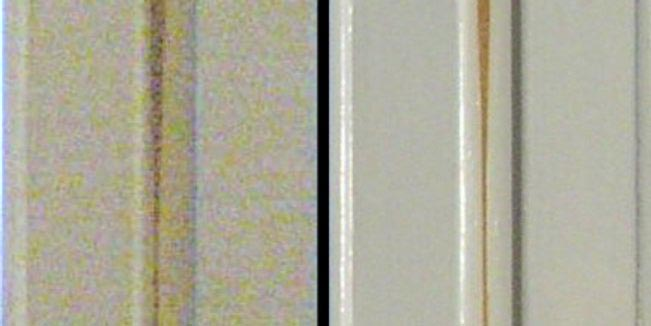
\includegraphics[width=\textwidth]{img/Noise_Comparison}
	\caption{Пример зашумленного изображения.}
	\label{fig:noise_compration}
\end{figure}

Также существуют изображения, полученные не только с фотосенсоров. Примером можно привести рентгенографию, широко используемую во многих областях, таких как медицина, процессы производства и эксплуатации, криминалистика, реставрация и экспертиза художественных ценностей. Существует два варианта получения цифрового изображения рентгенографии, это оцифровка уже существующего рентгеновского снимка, и использование технологии цифровой рентгенографии, при которой сразу идет цифровая обработка получаемого рентгеновского изображения. Оба данных метода подвержены наличию шума на получаемом цифровом изображении, в большей мере шум преобладает на изображених, получаемых первым способом, так как идёт дополнительное наложение шума сканирующим устройством. Пример подобного шума проиллюстрирован на изображении \ref{fig:reng_scan}. Аналогичная ситуация наблюдается и с снимками в области радиографического контроля сварных соединений, пример проиллюстрирован на изображении \ref{fig:reg_met_scan}.

\begin{figure}[h]
	\centering
	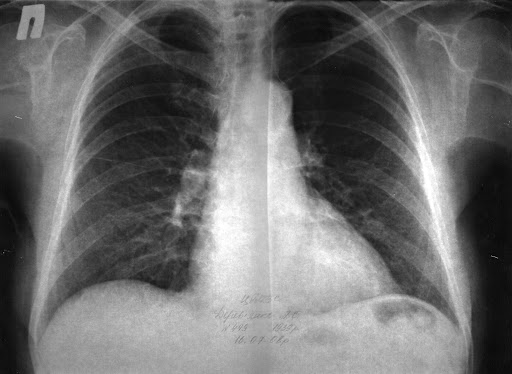
\includegraphics[width=\textwidth]{img/reng_scan}
	\caption{Сканированный рентгеновский снимок грудной клетки человека.}
	\label{fig:reng_scan}
\end{figure}

\begin{figure}[h]
	\centering
	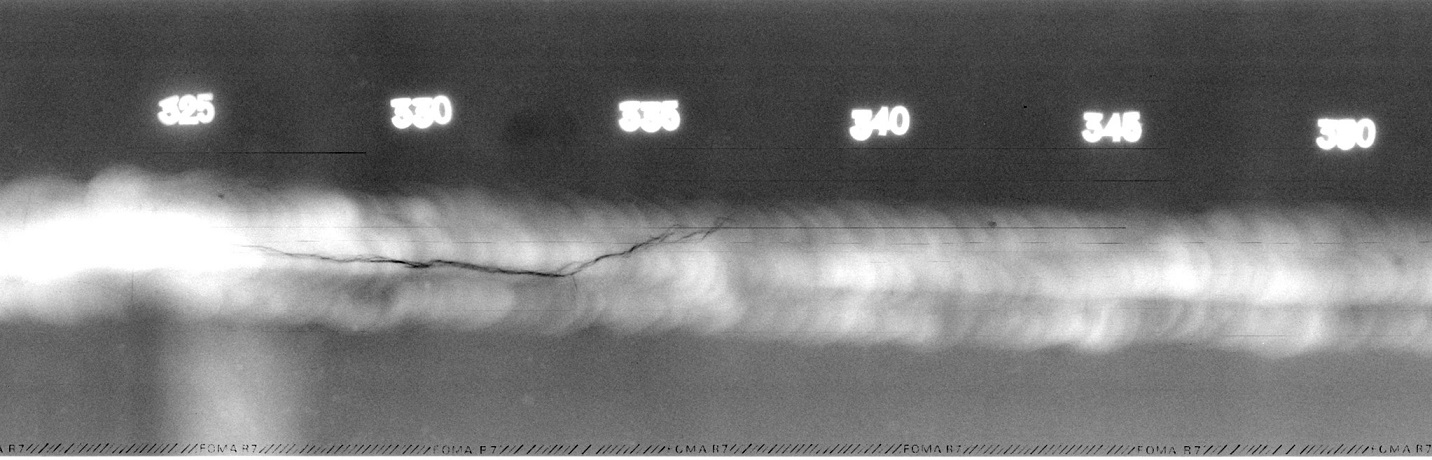
\includegraphics[width=\textwidth]{img/reng_met_scan}
	\caption{Цифровой рентгеновский снимок сварного соединения.}
	\label{fig:reg_met_scan}
\end{figure}

Помимо рентгенографии в обработке медицинских изображений потребность в избавлении полезного сигнала от шума встречаются и в других методах диагностики и визуализации, таких как цифровая реконструкция компьютерной томографии, магнитно-резонансной томографии и других. Потребность в шумоподавлении на медицинских цифровых изображениях изложена в работе~\autocite{MedicalImagesProcessing}.

На данный момент с развитием технологий глубокого обучения и построения глубоких архитектур сверточных нейронных сетей, такие архитектуры применяются к решению широкого ряда задач в области обработки и анализа изображений. Существует три подхода к обучению нейронных сетей: обучение с учителем, обучение без учителя и обучение с подкреплением. Если рассматривать близкие задачи к шумоподавлению с точки зрения построения шаблона обучения сети, это задача увеличения разрешения изображения с помощью нейронных сетей~\autocite{SuperResolutuion:journals/corr/abs-1807-02758} и задача восстановления изображения~\autocite{ImageReconstruction:journals/corr/abs-1903-10146}. Для решения данных задач нейросетевые архитектуры обучаются с помощью подхода обучения с учителем~\autocite{SupervisedLearningReview}. При процессе обучения таких архитектур в качестве входных данных выступают сжатые варианты изображений, подаваемых, как ожидаемые при предсказании сети. Если рассматривать в данном контексте обучение для задачи классификации, то на вход сети необходимо подавать изображение с присутствующем на нём шумом, и обучать сеть предсказывать уже само чистое изображение без шума. 

Все перечисленные способы в этом разделе получения цифрового изображения объединяет один недостаток, это невозможность получения чистого изображения без шума для обучения шумоподавляющей нейронной сети. В данной работе рассматривается подход к построению архитектуры шумоподавляющей нейронной сети и построения обучающего процесса, основанного на методе обучения без учителя (неконтролируемое обучение).

 %Обычно шум на изображении подавляется простыми алгоритмами, к примеру применением медианного фильтра или с помощью гауссова %сглаживания. Также существуют подходы, основанные на использовании нейронных сетей. Но главная проблема их применения заключается в %отсутствие данных для обучения. При обучении шумоподавляющей нейросети в качестве входных данных передаётся зашумленное изображение, а %в качестве ожидаемого ответа необходимо передавать «чистое» входное изображение без шума. В реальных задачах, как правило, нет таких пар %изображений. В данной работе рассматривается задача шумоподалвения цифрового шума.


\chapter{Задача шумоподавления}
\label{sec:init}

\section{Постановка задачи}
Пусть имеется изображение в формате непрерывного сигнала, полученного с АЦП об сигналах матрицы фотосенсора фиксированного цифрового устройства в момент времени $t$ (DNG формат~\autocite{DNG}):
\begin{equation}\label{eq:signal}
S(t)
\end{equation}

Сигнал $S(t)$~\ref{eq:signal} состоит из полезного сигнала $G(t)$ и шума $r(t)$, порождаемым фотосенсором:
\begin{equation}\label{eq:signal_decomposition}
S(t)\ =\ G(t)\ +\ r(t)
\end{equation}

При применении преобразования сырого сигнала $S(t)$ к трехмерному дискретному изображению в цветовой схеме RGB получаем матрицу изображения  $\tilde{I}$, с влиянием шума квантования при округлении сигнала при его дискретизации. Подход преобразования $p$ описан в работе Processing RAW Images in MATLAB~\autocite{RAWtoRGB}.
\begin{eqnarray}\label{eq:raw_image_matrix}
\tilde{I}_{i,j} = p(S(t))_{i, j}\ +\ q,\ q  \sim \mathcal{N}(-\frac{1}{2}, \frac{1}{12})\ \text{,}
\end{eqnarray}
где $q$, это шум квантования, семплируемый из нормального распределения с параметрами $\mathcal{N}(-\frac{Q}{2}, \frac{Q}{12})$ при шаге квантования $Q\ =\ 1$, более подробно можно ознакомиться с этим в главе Оценки ошибок (шумов) квантования выходного сигнала в цифровом фильтре из книги Цифровая обработка сигналов~\autocite{DSP}.

Для упрощения постановки задачи будем полагать, что матрица изображения $\tilde{I}$ состоит из суммы изображения, полученного из преобразования чистого (полезного) сигнала $G(t)$~\ref{eq:signal_decomposition} в матрицу $I$ и шума $\alpha$, полученного из случайного распределения $\mathbb{P}$, так как появление шума $r(t)$~\ref{eq:raw_image_matrix} можно считать абсолютно случайным процессом.
\begin{equation}\label{eq:matrix_def}
\tilde{I}\ =\ I\ +\ \alpha,\ \alpha \sim \mathbb{P}
\end{equation}

Таким образом, имея серию из $N$ изображений одной и той же сцены, снятых в разный момент времени $t$ имеем следующую выборку:
\begin{equation}\label{eq:collection}
\{\tilde{I}_k\}_{k=1}^{N}\text{ , где }\tilde{I_k}\ =\  I\ +\ \alpha_kjjjjjjjjjj\ \alpha_k \sim \mathbb{P}
\end{equation}
Причём для каждого элемента из набора $\tilde{I}_k$ компонента $I$ является одним и тем же значением, так как при съёмке одной сцены полезный сигнал $G(t)$~\ref{eq:signal_decomposition} остаётся неизменным.

Целью данной работы является построение с помощью нейронной сети приближения отображения $\phi: \mathbb{R}^n \longrightarrow \mathbb{R}^n$, обладающим следующим свойством:
\begin{equation}\label{eq:main_property}
\forall \tilde{I} \in \{\tilde{I}_k\}_{k=1}^{N} \Longrightarrow \phi(\tilde{I}) = I 
\end{equation}
Для построения приближения отображения $\phi$, нейронная сеть $f$ будет обучаться решать следующую задачу оптимизации:
\begin{eqnarray}\label{eq:main_min_task}
\min_{\mathnormal{w}} \Arrowvert f(\tilde{I}, \mathnormal{w}) - I \Arrowvert_{L_2}\text{ ,}
\end{eqnarray}
где $\mathnormal{w}$ - параметры сети $f$, $L_2$ - евклидова норма~\autocite{Haykin}.


\section{Анализируемые данные}
Изображения для проведения исследования были получены с помощью устройства \textit{Apple iPhone X}, имеющего камеру, состоящую из двух сенсоров.

\begin{table}[h!]
	\centering
	\caption{\label{tab:cam1}Характеристики первого сенсора}
	\begin{tabular}{llr}
		\toprule
		Характеристика  & Значение    & Единица измерения \\
		\midrule
		Разрешение & 12    & $MP$  \\
		Апертура & f/1.8 & \\
		Диагональ & 28 & $mm$ \\
		Размер сенсора & 1/3" & \\
		Размер пикселя & 1.22 & $\mu m$ \\
		Стабилизация изображения & OIS & \\
		\bottomrule
	\end{tabular}
\end{table}

\begin{table}[h!]
	\centering
	\caption{\label{tab:cam2}Характеристики второго сенсора}
	\begin{tabular}{llr}
		\toprule
		Характеристика  & Значение    & Единица измерения \\
		\midrule
		Разрешение & 12    & $MP$  \\
		Апертура & f/2.4 & \\
		Диагональ & 52 & $mm$ \\
		Размер сенсора & 1/3.4" & \\
		Размер пикселя & 1.0 & $\mu m$ \\
		Стабилизация изображения & OIS & \\
		\bottomrule
	\end{tabular}
\end{table}

С данного устройства были сделаны серии изображений семи сцен с различным освещением и цветовым наполнением. Данные серии получены стандартными средствами для съёмки на устройстве. Под сценой подразумевается съёмка неизменяемой картины реального мира, получая матрицу~\ref{eq:matrix_def}. Для этого устройство фиксировалось на штативе в неподвижном состоянии  и запуск процесса съёмки кадра производился  с беспроводного устройства, тем самым получая набор изображений $\{\tilde{I}^q_k\}_{k=1}^{N}$~\ref{eq:collection}, где $q$ - порядковый номер снимаемой сцены.

% 95 фотографий
Каждая сцена содержит в среднем по $14$ фотографий, суммарное количество кадров из всех наборов составляет $95$ изображений.


Так как стандартные средства для съёмки не позволяют получать RAW (изображение с сырого сигнала АЦП~\ref{eq:signal}) изображение, то были произведены съёмки дополнительных сцен с использованием стороннего программного обеспечения, позволяющего получать <<сырые>>  кадры в формате TIFF~\autocite{TIFFArticle}: ~\href{https://apps.apple.com/ru/app/simple-raw-camera/id1286921686}{Simple Raw camera}, ссылка на приложение~\url{https://apps.apple.com/ru/app/simple-raw-camera/id1286921686}


% Если typeOfWork в SETUP.tex задан как 2 или 3, то начинать
% надо не с section (раздел), а с главы (chapter)
\section{Несколько примеров в~\LaTeX{}}
\label{sec:examples}

Некоторые часто используемые
команды приведены в качестве примера ниже (и варианты — в
комментариях). Мы рекомендуем внимательно прочесть данный
текст и изучить его исходный код прежде, чем начинать писать
свой собственный. Кроме того, можно дать и такой совет: идущий
ниже текст не убирать до самого конца, а просто оставлять его
позади своего собственного текста, чтобы в любой момент можно
было проконсультироваться с данными примерами.

\subsection{Как вставлять листинги и рисунки}

Для крупных листингов есть два способа. Первый красивый, но в нём не допускается
кириллица (у вас может встречаться в комментариях и
печатаемых сообщениях), он представлен на листинге~\ref{list:hwbeauty}.
\begin{ListingEnv}[H]% буква H означает Here, ставим здесь,
% элементы, которые нежелательно разрывать обычно не ставят
% посреди страницы: вместо H используется t (top, сверху страницы),
% или b (bottom) или p (page, на отдельной странице)
\begin{lstlisting}
#include <iostream>
using namespace std;

int main()
{
    cout << "Hello, world" << endl;
    system("pause");
    return 0;
}
\end{lstlisting}
%следующую команду для генерации подписи можно опустить,
% хотя рекомендуется все специальные элементы (таблицы, рисунки,
% листинги) подписывать. Если подпись пропустить, листинг также не получит
% номера и на него не сошлёшься в будущем
\caption{Программа “Hello, world” на \protect\cpp}
% далее метка для ссылки:
\label{list:hwbeauty}
\end{ListingEnv}

Второй не такой красивый, но без ограничений (см.~листинг~\ref{list:hwplain}).
\begin{ListingEnv}[H]
\begin{Verb}

#include <iostream>
using namespace std;

int main()
{
    cout << "Привет, мир" << endl;
}
\end{Verb}
\caption{Программа “Hello, world” без подсветки}
\label{list:hwplain}
\end{ListingEnv}

Можно использовать первый для вставки небольших фрагментов
внутри текста, а второй для вставки полного
кода в приложении, если таковое имеется.

Если нужно вставить совсем короткий пример кода (одна или две строки), то выделение  линейками и нумерация может смотреться чересчур громоздко. В таких случаях можно использовать окружения \texttt{lstlisting} или \texttt{Verb} без \texttt{ListingEnv}. Приведём такой пример с указанием языка программирования, отличного от заданного по умолчанию:
\begin{lstlisting}[language=Haskell]
fibs = 0 : 1 : zipWith (+) fibs (tail fibs)
\end{lstlisting}
Такое решение~--- со вставкой нумерованных листингов покрупнее
и вставок без выделения для маленьких фрагментов~--- выбрано,
например, в книге Эндрю Таненбаума и Тодда Остина по архитектуре
компьютера~\autocite{TanAus2013} (см.~рис.~\ref{fig:tan-aus}).

Наконец, для оформления идентификаторов внутри строк
(функция \lstinline{main} и тому подобное) используется
\texttt{lstinline} или, самое простое, моноширинный текст
(\texttt{\textbackslash texttt}).

\begin{figure}[p]% p означает, что нужно выделить для рисунка
% отдельную страницу; применяется для больших рисунков
\centering
%Здесь могла быть ваша лягушка.
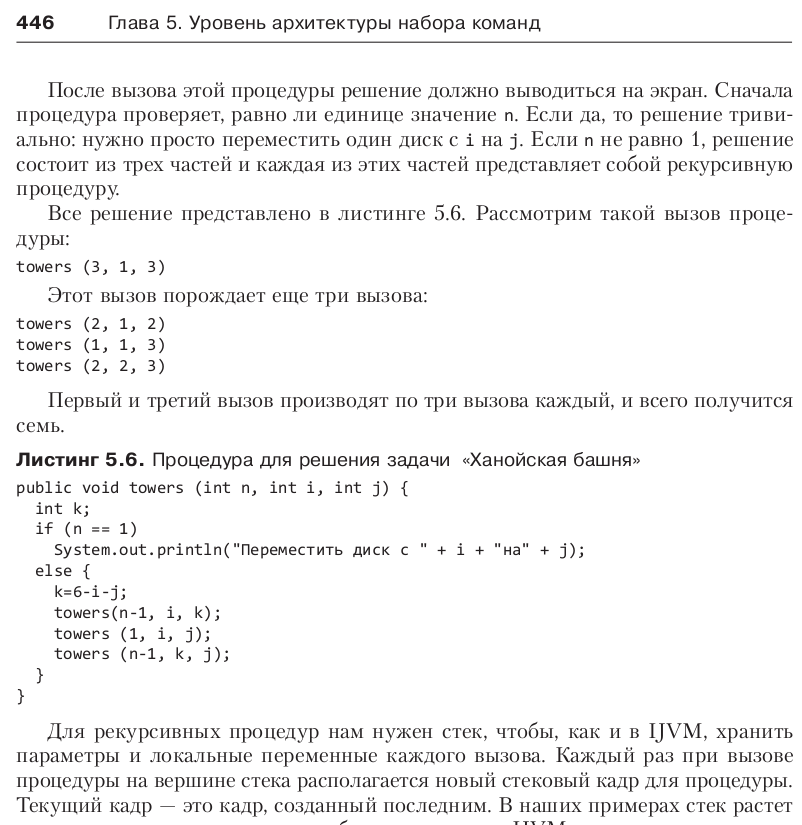
\includegraphics[width=\textwidth]{img/tan-aus.png}
\caption{\label{fig:tan-aus}Пример оформления листингов в~\autocite{TanAus2013}}
\end{figure}

Использовать внешние файлы (например, рисунки) можно и на \href{http://overleaf.com}{overleaf.com}: ищите кнопочку upload.

\subsection{Как оформить таблицу}

Для таблиц обычно используются окружения table и tabular --- см. таблицу~\ref{tab:widgets}. Внутри окружения tabular используются специальные команды пакета booktabs — они очень красивые; самое главное: использование вертикальных линеек считается моветоном.

\begin{table}
\centering
\caption{\label{tab:widgets}Подпись к таблице --- сверху}
\begin{tabular}{llr}
\toprule
\multicolumn{2}{c}{Item} \\
\cmidrule(r){1-2}
Животное  & Описание    & Цена (\$) \\
\midrule
Gnat      & per gram    & 13.65      \\
          & each        & 0.01       \\
Gnu       & stuffed     & 92.50      \\
Emu       & stuffed     & 33.33      \\
Armadillo & frozen      & 8.99       \\
\bottomrule
\end{tabular}
\end{table}

\subsection{Как набирать формулы}

\LaTeX{} is great at typesetting mathematics. Let $X_1, X_2, \ldots, X_n$ be a sequence of independent and identically distributed random variables with $\text{E}[X_i] = \mu$ and $\text{Var}[X_i] = \sigma^2 < \infty$, and let
$$S_n = \frac{X_1 + X_2 + \cdots + X_n}{n}
      = \frac{1}{n}\sum_{i}^{n} X_i$$
denote their mean. Then as $n$ approaches infinity, the random variables $\sqrt{n}(S_n - \mu)$ converge in distribution to a normal $\mathcal{N}(0, \sigma^2)$.

\subsection{Как оформлять списки}

Нумерованные списки (окружение enumerate, команды item)…

\begin{enumerate}
  \item Like this,
  \item and like this.
\end{enumerate}

\dots маркированные списки \dots

\begin{itemize}
  \item Like this,
  \item and like this.
\end{itemize}

\dots списки-описания \dots

\begin{description}
  \item[Word] Definition
  \item[Concept] Explanation
  \item[Idea] Text
\end{description}

\Conc

Помните, что на все пункты списка литературы должны быть ссылки. \LaTeX\ просто не добавит информацию об издании из bib"/файла, если на это издание нет ссылки в тексте. Часто студенты используют в работе  электронные ресурсы: в этом нет ничего зазорного при одном условии: при каждом заимствовании следует ставить соответствующую ссылку. В качестве примера приведём ссылку на сайт нашего института~\autocite{mmcs}.

Для дальнейшего изучения \LaTeX\ рекомендуем книгу Львовского~\autocite{Lvo2003}: она хорошо написана, хотя и несколько устарела.
Обычно стоит искать подсказки на
\href{http://tex.stackexchange.com/}{tex.stackexchange.com}, а также
читать документацию по установленным пакетам с помощью
команды
\begin{Verb}
texdoc имя_пакета
\end{Verb}
или на \href{http://ctan.org/}{ctan.org}.

% Печать списка литературы (библиографии)
\printbibliography[%{}
    heading=bibintoc%
    %,title=Библиография % если хочется это слово
]
% Файл со списком литературы: biblio.bib
% Подробно по оформлению библиографии:
% см. документацию к пакету biblatex-gost
% http://ctan.mirrorcatalogs.com/macros/latex/exptl/biblatex-contrib/biblatex-gost/doc/biblatex-gost.pdf
% и огромное количество примеров там же:
% http://mirror.macomnet.net/pub/CTAN/macros/latex/contrib/biblatex-contrib/biblatex-gost/doc/biblatex-gost-examples.pdf

\end{document}
